\chapter{Interactions}


Dans le but de décrire la collaboration entre les composants et les contraintes de ceux-ci, il est important de montrer quelques exemples de scénarios : \\

\begin{itemize}
\item Connexion au serveurs
\item Manipulation de données 
\item Synchronisation entre les serveurs
\end{itemize}

%Décrire, à haut-niveau, la collaboration entre les composants majeurs, en faisant référence aux besoins.
%Utiliser des interactions, c'est à dire, des diagrammes de séquence et des diagrammes de communication. Utiliser éventuellement des diagrammes d'activités.
%\emph{Ne vous limitez pas à une seule interaction par cas d'utilisation}

\section{Connexion au serveurs}


Le scénario suivant mets en évidence la connexion du clientWeb aux serveurs GTD et ToodleDo. La gestion des connexions est assurée par le composant ConnectionManager. C'est également lui qui va gérer les sessions utilisateurs. Comment on peut le voir, l'objet session va stocker les informations relatives aux connexions sur les serveurs GTD et ToodleDo (couple login/password notamment). Celui ci sera envoyé au DataManager qui va se connecter aux serveurs GTD et ToodleDo.


\begin{figure}[H]
  \begin{center}
  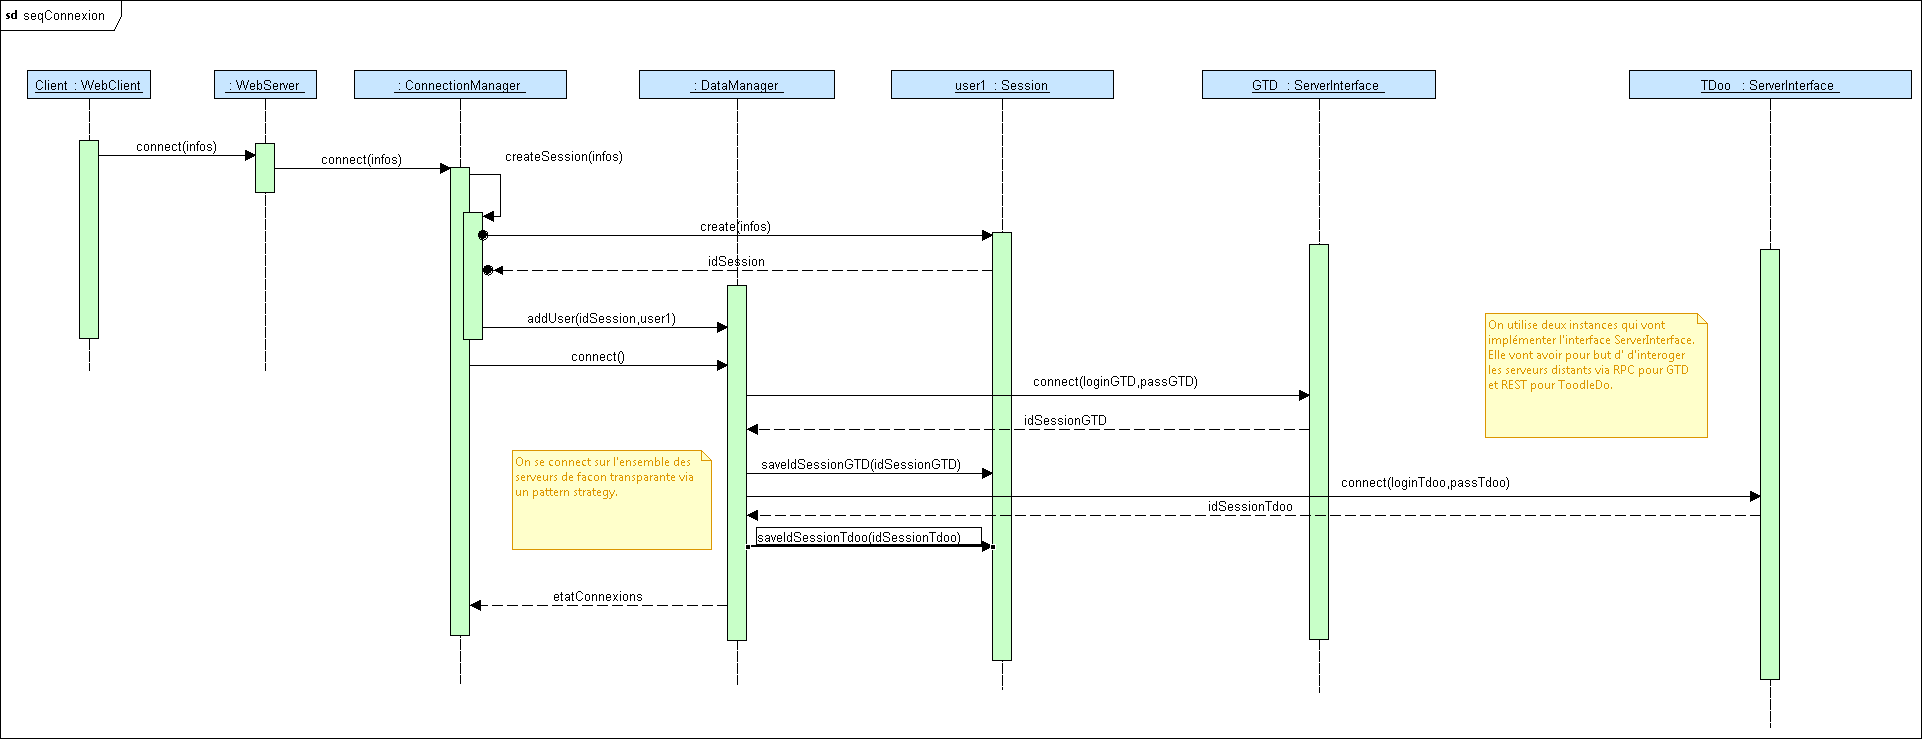
\includegraphics[scale=0.4,angle=90]{livrable3/images/connection.png}
  \caption{UML - Diagramme de séquences - Connexion au serveurs}
  \end{center}
\end{figure}


\section{Affichage des projets}


\begin{figure}[H]
  \begin{center}
  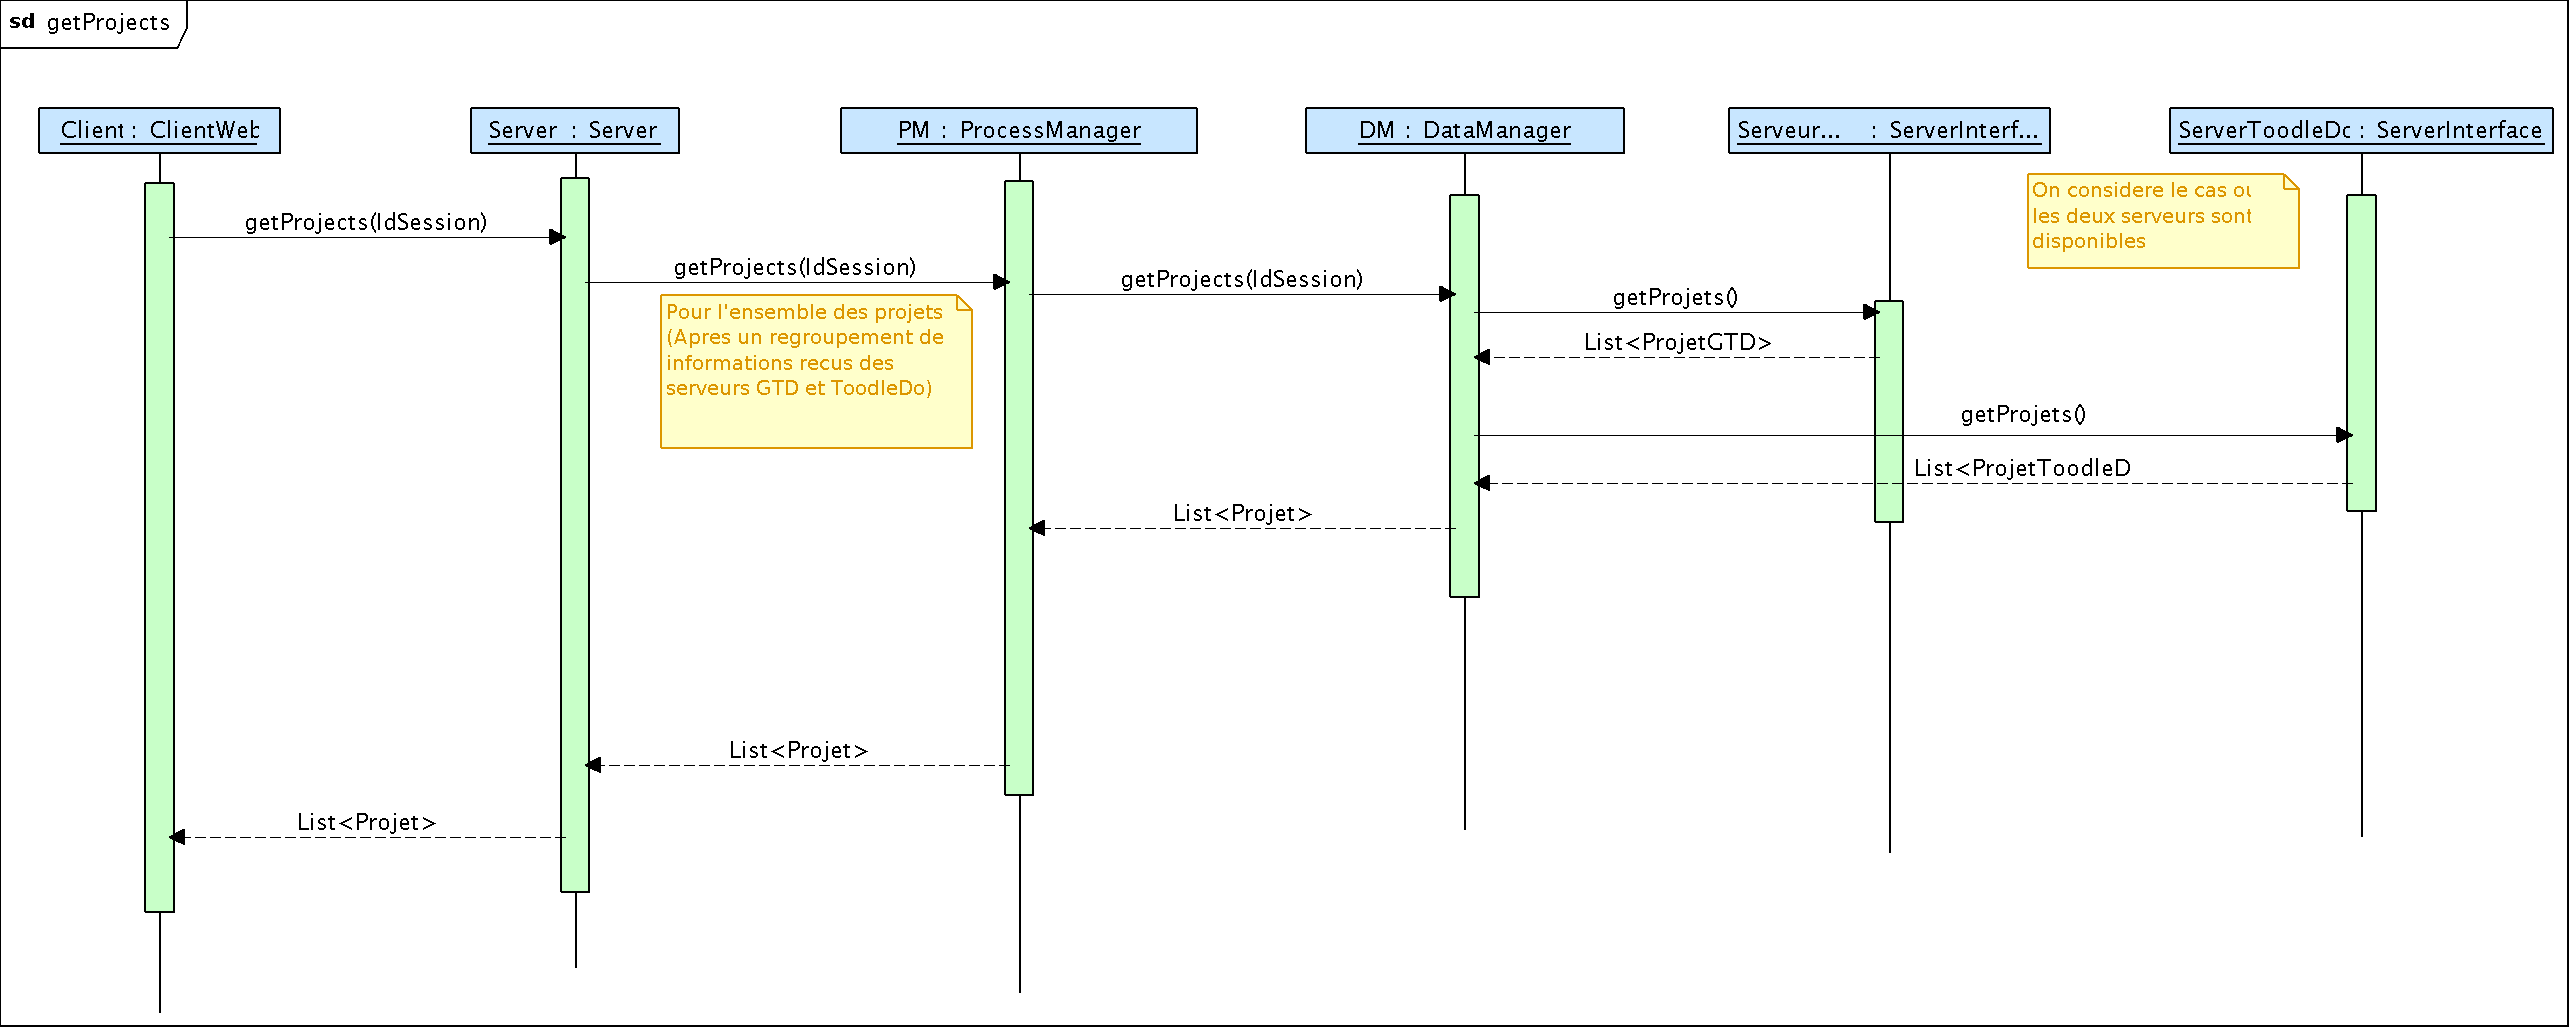
\includegraphics[scale=0.25,angle=90]{livrable3/images/display.png}
  \caption{UML - Diagramme de séquences - Affichage des projets}
  \end{center}
\end{figure}



\section{Synchronisation}

Le processus de synchronisation permet d'avoir des données identiques sur les serveurs GTD et ToodleDo (après une indisponibilité d'un serveur par ex). Dans le scénario suivant, l'utilisateur récupère une liste de projets. Le DataManager qui assure la transparence lors de la récupération des projets, s'aperçoit que les listes sont différentes (il manque un projet sur le serveur ToodleDo). Il va donc ajouter le projet manquant sur le serveur ToodleDo. En ce qui concerne la synchronisation il faut prendre en considération que le serveur GTD est le serveur maitre de l'application. 

\begin{figure}[H]
  \begin{center}
  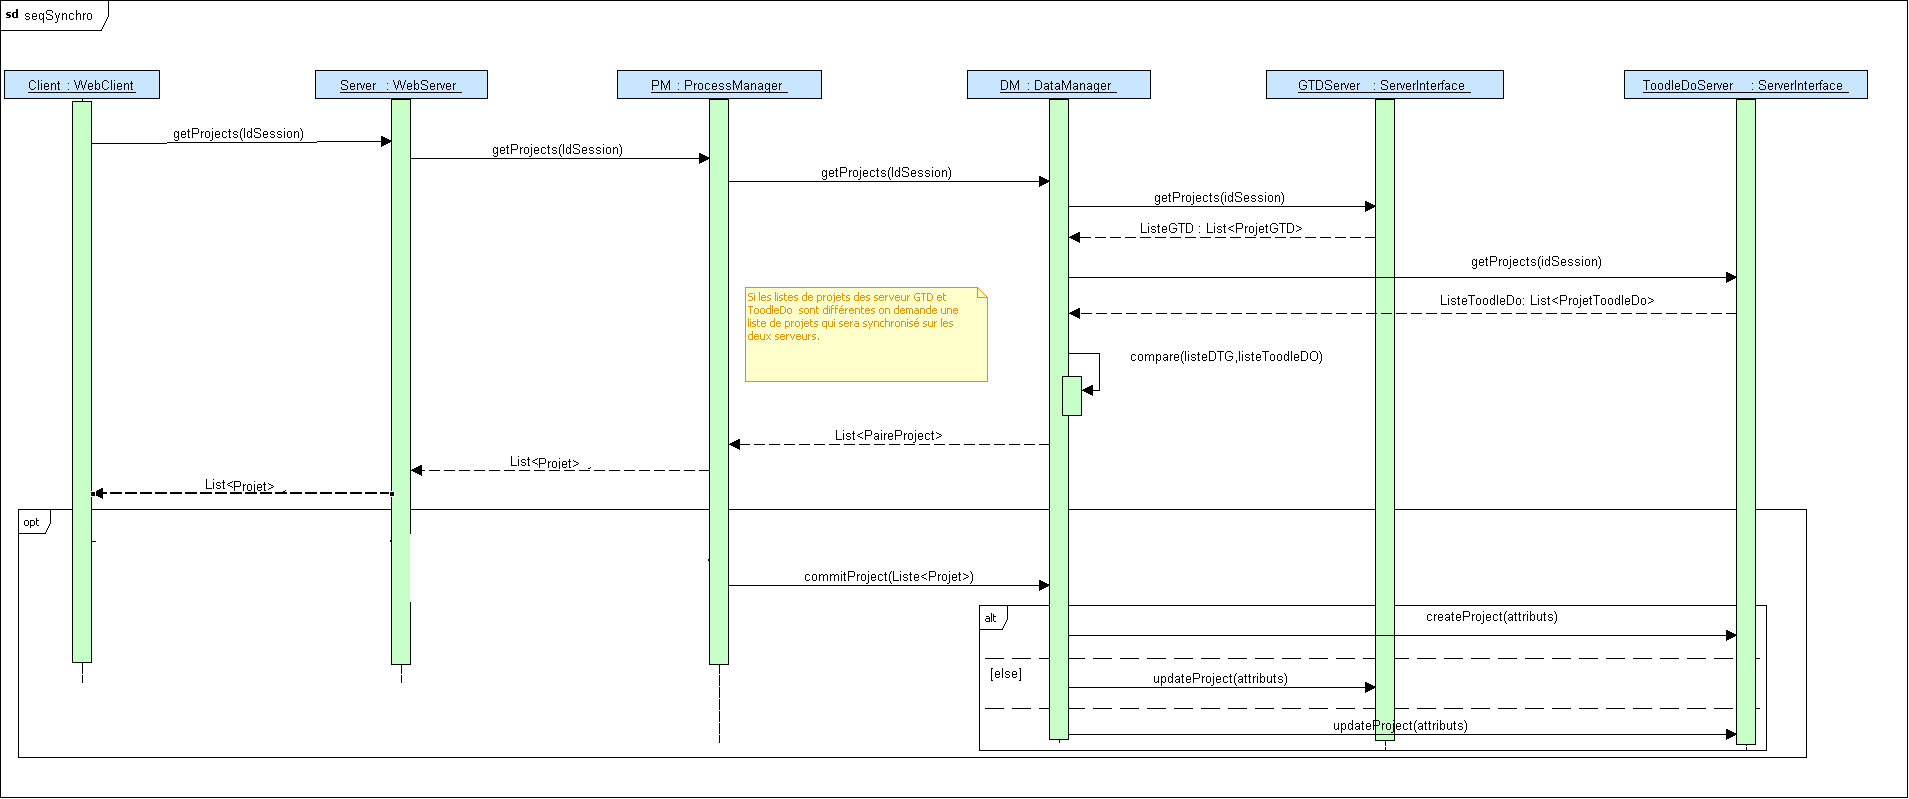
\includegraphics[scale=0.25,angle=90]{livrable3/images/synchro.png}
  \caption{UML - Diagramme de séquences - Synchronisation}
  \end{center}
\end{figure}

